\section{Invariant subspaces}
\lettrine{C}{onsider}
a linear operator \( T \in \lmap(\vsV) \), where \(\vsV\) is a finite dimensional vector space.
For any subspace \(\vsS \subset \vsV\) the image of \(T\) over \(\vsS\) is, in general, some other arbitrary subspace.
It is natural then to want to consider subspaces which preserve their structure under \( T \). The following definition captures this idea.
\begin{definition}
    A subspace \( \vsS \) is called \textit{invariant} under the linear map \( T \) if

    \begin{equation*}
        \vv \in \vsS \implies T\vv\in \vsS
    \end{equation*}
\end{definition}


It is best to give some examples of such subspaces before investigating them further:

\subsection{Examples and properties}

\begin{example}
    The subspace called the eigenspace of \(T\) at eigenvalue \(\lambda\)
    \begin{equation*}
        E_\lambda = \{\vv: T\vv=\lambda \vv\}
    \end{equation*}

    is invariant - each element is scaled under \(T\), which is still in \(E_\lambda\).
\end{example}


\begin{example}\label{ex:invariance_image}
    The image

    \begin{equation*}
        \im T=\{T\vv: \vv\in\vsV\}
    \end{equation*}

    is invariant by definition:
    \begin{equation*}
        \vv\in T(\vsV)\implies T\vv\in T(\vsV)
    \end{equation*}
\end{example}

\begin{example}\label{ex:invariance_ext_kernel}
    The generalized kernel

    \begin{equation*}
        K=\{\vv: \exists k\in \N \text{ s.t } T^k\vv=\0\}
    \end{equation*}

    is invariant under \( T \).
    This is indeed a subspace, and the invariance here follows from its definition.
    \begin{equation*}
        \vv\in K \implies \exists k,\; T^k\vv=\0 \implies T^{k-1}T\vv=\0 \implies T\vv\in K
    \end{equation*}

    This set has a stronger structure than being just invariant. It can be seen that
    \begin{equation}
        \vv\notin K\implies T\vv\notin K \label{eq:initial}
    \end{equation}
    which is not in general true for invariant subspaces.
\end{example}


\begin{figure}
    \centering
    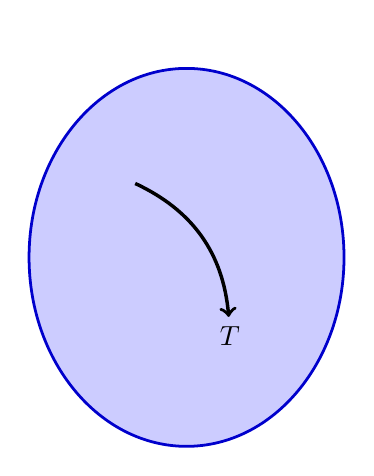
\begin{tikzpicture}[scale=2]
        \draw[
            fill=blue!20,
            draw=blue!80!black,
            line width=1pt
        ] (0,0) ellipse [x radius=1cm, y radius=1.2cm];

        \node [right] (A) at (-0.45,0.5) {\( \vv \)};
        \node [right] (B) at (0.15,-0.5) {\( T\vv \)};
        \node at (0, 1.4) {\( \vsS \)};

        \draw[->, line width=1.25pt] (A) to[bend left=30] (B);

    \end{tikzpicture}
    \caption{A subspace \( \vsS \) invariant  under \(T\)}
\end{figure}

Because of their behavior, we want to search for building blocks of \( \vsV \) of invariant subspaces - similarly to how primes are building blocks of the integers.
By building blocks, we mean invariant subspaces

\begin{equation*}
    \vsS_1,\vsS_2,...,\vsS_\sigma
\end{equation*}

such that given basis \(\beta_i\) for \(\vsS_i\), we have
\begin{equation*}
    \beta = \bigcup_{i=1}^\sigma \beta_i
\end{equation*}
is a basis for \( \vsV \).

Equivalently,
\begin{equation*}
    \bigoplus_{i=1}^\sigma\vsS_i=\vsV
\end{equation*}

If we one succeeds in this, then there would be a matrix representation of \(T\) in the form

\begin{equation*}
    {}_\beta[T]_\beta =
    \begin{pmatrix}
        A_1    & 0      & \cdots & 0      \\
        0      & A_2    & \cdots & 0      \\
        \vdots & \vdots & \ddots & \vdots \\
        0      & 0      & \cdots & A_\sigma
    \end{pmatrix}
\end{equation*}

This structure is strictly due to the invariance of the subspaces - if \(\beta_i\) is a basis for \( \vsS_i \) consisting of \(\beta_{i1},\beta_{i2},...,\beta_{ik}\), then

\begin{equation*}
    T(\beta_{ij})\in \vsS_i\ \forall j\leq k,
\end{equation*}

and therefore may be expressed only in terms of \(\beta_{i1},\beta_{i2},...,\beta_{ik}\) - hence the above pattern.

\vspace{\baselineskip}

Our goal is to achieve this decomposition with choosing the best possible invariant subspaces - so that the above \(A_i\) blocks are of the simplest scheme.

It should already be obvious which invariant subspaces to start from. Before continuing, some properties:


\begin{property}
    Invariant subspaces (except \(\{\0\}\)) \(\vsS\) under \(T\) all contain an eigenvector of \(T\). This is for the reason that the linear map

    \begin{equation*}
        T^*:\vsS\rightarrow \vsS\ \text{,} \ T^*\vv=T\vv
    \end{equation*}

    is well defined due to the invariance. Then we just pick the eigenvector of \( T^* \) (always exists).

\end{property}

\begin{lemma}\label{lem:invariance_sum}
    If \(\vsS\) is invariant under \(T\) and \(L\), then \(\vsS\) is invariant under \(T+xL\) for any \(x\in\C\).
\end{lemma}
\begin{proof}
    If \(\vv\in\vsS\), then
    \begin{equation*}
        (T+xL)\vv = T\vv+xL\vv \in \vsS
    \end{equation*}
\end{proof}

\begin{lemma}\label{lem:invariance_power}
    If \(\vsS\) is invariant under \(T\) then \(\vsS\) is also invariant under \(T^n\) for any \(n\in\N\).
\end{lemma}
\begin{proof}
    The statement is true for \(n=0\), as
    \begin{equation*}
        T^0(\vsS)=\id(\vsS)=\vsS\subseteq\vsS
    \end{equation*}

    If the statement is true for some \(n\),
    \begin{equation*}
        T^{n+1}(\vsS)=T(T^n(\vsS))\subseteq T(\vsS) \subseteq \vsS
    \end{equation*}

    So by induction, the statement is true.
\end{proof}

\begin{corollary}\label{col:invariant_poly}
    If \(\vsS\) is invariant under \(T\), then it is also invariant under any polynomial of \(T\).
\end{corollary}

% \begin{lemma}\label{lem:invariance2}
%     \begin{equation*}
%         \vsS\ \text{invariant under } T\iff \vsS\ \text{invariant under } T-x\id\ \forall x\in \C,
%     \end{equation*}

%     and consequently invariant under any polynomial \(P(T)\).
% \end{lemma}

\section{The Jordan form}


\subsubsection{Statement}
For a linear operator \(T \in \lmap(\vsV)\) where \(\vsV\) is finite dimensional, there is a matrix representation of \(T\) of the form
\begin{equation*}
    \begin{pmatrix}
        J_1    & 0      & \cdots & 0      \\
        0      & J_2    & \cdots & 0      \\
        \vdots & \vdots & \ddots & \vdots \\
        0      & 0      & \cdots & J_k
    \end{pmatrix}
\end{equation*}

where \(J_i\) is a square matrix of the form

% Note:
% Question: are the k blocks meant to be jordan block or jordan matrix of each eigenvalue?

\begin{equation*}
    \begin{pmatrix}
        \lambda    & 1      & \cdots & 0      \\
        0      & \lambda    & \cdots & 0      \\
        \vdots & \vdots & \ddots & 1 \\
        0      & 0      & \cdots & \lambda
    \end{pmatrix}
\end{equation*}


\subsection{Method}
We start with considering the simplest invariant subspaces - the eigenspaces.
For some \(T\in\lmap(\vsV)\), let the spectrum of \(T\) be \(\{\lambda_1, \lambda_2,...,\lambda_\sigma\}\), and define the corresponding eigenspaces

\begin{equation*}
    E_{\lambda_{i}}=\{\vv\in\vsV: T\vv=\lambda_i \vv\}
\end{equation*}

It is important to note that

\begin{equation*}
    E_{\lambda_i}\cap E_{\lambda_j}=\{\0\}  \ \text{, for all }i\neq j\leq k,
\end{equation*}

and that for an arbitrary basis \(\beta_i\) for \(E_{\lambda_i}\), the set

\begin{equation*}
    \bigcup_{i=1}^{\sigma} \beta_i
\end{equation*}

is linearly independent.

\begin{figure}[H]
    \centering
    \begin{tikzpicture}[scale=2]
        \foreach \angle/\color/\labeltext in {0/blue/\(E_{\lambda_1}\), 120/teal/\(E_{\lambda_2}\), 240/purple/\(E_{\lambda_3}\)} {
                \begin{scope}[rotate=\angle]
                    \draw[fill=\color!20, draw=\color!80!black, line width=1pt]
                    (0,1.5) .. controls (-0.7,1.4) and (-0.8,0.6) .. (0,0)
                    .. controls (0.8,0.6) and (0.7,1.4) .. (0,1.5) -- cycle;
                    \node[ font=\bfseries\sffamily] at (0,0.8) {\labeltext};
                \end{scope}
                \node[
                    below right,          % Position relative to (0,0)
                    font=\small\sffamily  % Clean font style
                ] at (0,0) {\(\0\)};
            }
    \end{tikzpicture}
    \caption{Three eigenspaces of some map \(T\)}
\end{figure}


Is \(\bigoplus_{i=1}^{\sigma} E_{\lambda_i} = \vsV\) true? - if yes, \(\bigcup \beta_i\) may be our basis.

Sadly, this is often not the case.
An example is the matrix
\begin{equation*}
    A = \begin{pmatrix}
        1 & 1 & 0 \\
        0 & 1 & 1 \\
        0 & 0 & 1
    \end{pmatrix}
\end{equation*}
with its corresponding linear map.

If \(\bigoplus E_{\lambda_i}\) is not enough to cover \(\vsV\), we want to somehow expand each \(E_{\lambda_i}\) into a bigger subspace, with the importance to keep their invariance and disjointedness.


\subsection{Generalising the eigenspaces}

For each \(E_{\lambda_i}\), denote

\begin{equation*}
    \Gi^{k}=\ker(T-\lambda_i\id)^k
\end{equation*}

Note that \(\Gi^1=E_{\lambda_i}\) and \(\Gi^{k}\subseteq\Gi^{k+1}\).

We will define
\begin{equation*}
    \boxed{
        \Gi=\bigcup_{k=1}^{\infty} \Gi^k
    }
\end{equation*}

Intuitively this can be thought of as extending the subspace to include vectors that are 'close' to becoming eigenvectors.
In the sense that they are a finite number of iterations of \(T- \lambda_i\id\) away from \(\0\).

However, we still have to show that this is a valid choice.
More specifically, we need to show that each \(\Gi\) is invariant under \(T\), and
\begin{equation*}
    \bigoplus_{i=1}^\sigma\Gi=\vsV
\end{equation*}


\subsection{Showing the subspaces works}

The definition of the extended eigenspace uses infinity as upperbound.
However, infinity is tricky to works with sometimes, so we provide the following lemma:

\begin{lemma} \label{lem:conv}
    For any \(\lambda_i\in\spec T\), there exists \(\kappa_i\in\N\) s.t. for any \(\kappa_i\le k\in\N\), we have \(\Gi=\Gi^{k}=\Gi^{\kappa_i}\).
\end{lemma}
\begin{proof}
    Since \(\Gi^{k}\) is a subspace of \(\vsV\) and \(\Gi^{k}\subseteq\Gi^{k+1}\), \((\dim\Gi^{k})_{k\in\N}\) is a monotone integer sequence bounded by \(\dim\vsV\).
    Hence, there exists some \(\kappa_i\in\N\) s.t. \(\dim\Gi^k=\dim\Gi^{\kappa_i}\) for all \(k\ge\kappa_i\).

    Since for all \(k\ge\kappa_i\), \(\Gi^k\supseteq\Gi^{\kappa_i}\), we have \(\Gi^k=\Gi^{\kappa_i}\).
    \begin{equation*}
        \Gi=\bigcup_{k=1}^{\infty}\Gi^k=\Gi^{\kappa_i}\cup\bigcup_{k=1}^{\kappa_i-1}=\Gi^{\kappa_i}
    \end{equation*}
\end{proof}

\begin{figure}[H] \label{fig:geneigen}
\centering
    \begin{tikzpicture}
        % (horizontal radius, vertical radius)
        \foreach \a/\clr/\b in {
            2.0/blue/4,
            1.5/teal/3,
            1.0/purple/2
        }{
            \draw[thick, fill=\clr!20, draw=\clr!80!black, line width=1pt] (0,\b) ellipse [x radius=1.5 * \a, y radius=\b];
        }
        \node[above] at (0, 2) {\(E_{\lambda_i}\)};
        \node[above] at (0, 5) {\(\ker (T - \lambda _i\id)^{2}\)};
        \node[above] at (0, 7) {\(\ker (T - \lambda _i\id)^{3}\)};

        \node[below] at (0,0) {\( \0 \)};
        % optional coordinate marker
        \fill (0,0) circle (1.5pt);
    \end{tikzpicture}
    \caption{The generalised eigenspace \( \Gi \) of the eigenvalue \(\lambda _i\). In this case \( \Gi \) stops growing at \(\ker (T - \lambda _i\id)^{3} \).}
\end{figure}

With this, we can show:
\begin{lemma} \label{lem:Gi_invariance}
    \(\Gi\) is invariant under any polynominal of \(T\).
\end{lemma}
\begin{proof}
    \(\Gi\) is the extended kernel of \(T-\lambda_i\id\).
    From example \ref{ex:invariance_ext_kernel}, we have \(\Gi\) is invariant under \(T-\lambda_i\id\).

    Applying lemma \ref{col:invariant_poly}, we have \(\Gi\) is invariant under \(T=T-\lambda_i\id+\lambda_i\id\) and thus, any polynominal of \(T\).
\end{proof}

\begin{corollary} \label{col:Gi_invariance}
    Noteably, \(\Gi\) is invariant under \(T-x\id\) for any choice of \(x\in\C\).
\end{corollary}

However, we can go one step further.
Since \(\Gi\) is invariant under \(T-x\id\), \(T-x\id\) is a well-defined function on \(\Gi\).
We claim
\begin{lemma} \label{lem:bijection}
    For all \(x\neq\lambda_i\in\C\), \(T-x\id\) is a bijection on \(\Gi\)
\end{lemma}
\begin{proof}
    From lemma \ref{lem:conv}, there exists
    \begin{align*}
        \ker_{\Gi}(T-x\id)
        &=\{\vv\in\Gi:(T-x\id)\vv=\0\}\\
        &=\{\vv\in\vsV:T\vv=x\vv \land (T-\lambda_i\id)^{\kappa_i}\vv=\0\}\\
    \end{align*}
    Note that since $T\vv=x\vv$,
    \begin{equation*}
        (T-\lambda_i\id)\vv=T\vv-\lambda_i\vv=(x-\lambda_i)\vv
    \end{equation*}
    where \(x-\lambda_i\neq0\) from the assumption. \\
    Hence,
    \begin{align*}
        \ker_{\Gi}(T-x\id)
        &=\{\vv\in\vsV:T\vv=x\vv \land (x-\lambda_i)^{\kappa_i}\vv=\0\}\\
        &\subseteq\{\vv\in\vsV:(x-\lambda_i)^{\kappa_i}\vv=\0\}\\
        &=\{\vv\in\vsV:\vv=\0\}\\
        &=\{\0\}\\
    \end{align*}
    Since \(\Gi\) has finite dimension, \(T-x\id\) is a bijection on \(\Gi\).
\end{proof}


\begin{lemma}
    \label{lem:img_sum_ker}
    \begin{equation*}
        \ker(T-\lambda_i\id)^{\kappa_i}\oplus\im(T-\lambda_i\id)^{\kappa_i}=\vsV
    \end{equation*}
    where \(\kappa_i\) is as defined in lemma \ref{lem:conv}.
\end{lemma}
\begin{proof}
    First, we will show that the two vector spaces are disjoint.

    Suppose $\vv \in \im(T-\lambda_i\id)^{\kappa_i}$, then there exist $\vu\in\vsV$ s.t. $\vv=(T-\lambda_i\id)^{\kappa_i}\vu$.
    Since $\vv\in\ker(T-\lambda_i\id)^{\kappa_i}$,
    \begin{align*}
        (T-\lambda_i\id)^{2\kappa_i}\vu
        &=(T-\lambda_i\id)^{\kappa_i}\left((T-\lambda_i\id)^{\kappa_i}\vu\right)\\
        &=(T-\lambda_i\id)^{\kappa_i}\vv\\
        &=\0
    \end{align*}
    Hence, $\vu\in\extker(T-\lambda_i\id)=\ker(T-\lambda_i\id)^{\kappa_i}$.
    \begin{equation*}
        \vv = (T-\lambda_i\id)^{\kappa_i}\vu = \0
    \end{equation*}
    Therefore, $\ker(T-\lambda_i\id)^{\kappa_i}\cap\im(T-\lambda_i\id)^{\kappa_i}=\{\0\}$.

    Since the two vector spaces are disjoint, they are also independent.
    Therefore,
    \begin{align*}
        &\dim\left(\ker(T-\lambda_i\id)^{\kappa_i}\oplus\im(T-\lambda_i\id)^{\kappa_i}\right)\\
        =&\dim\ker(T-\lambda_i\id)^{\kappa_i} + \dim\im(T-\lambda_i\id)^{\kappa_i}\\
        =&\dim\vsV\\
    \end{align*}
    by the dimension theorem.
    Hence, $\ker(T-\lambda_i\id)^{\kappa_i}\oplus\im(T-\lambda_i\id)^{\kappa_i}=\vsV$.
\end{proof}



\begin{theorem}
    \(\vsG_{\lambda_1}\oplus\vsG_{\lambda_2}\oplus\dots\oplus\vsG_{\lambda_\sigma}=\vsV\)
\end{theorem}
\begin{proof}
    Note that \(\{\0\}\oplus\vsG=\vsG\). So for \(\sigma=0\), we will define \(\vsG_{\lambda_1}\oplus\dots\oplus\vsG_{\lambda_\sigma}=\{\0\}\).

    If \(k=0\), since for any \(n\)-dimensional vector space \(\vsV\) where \(n > 0\), there exists eigenvalues for \(T\), we have \(n=0\).
    Thus, \(\vsV=\{\0\}\) and the theorem holds.

    Suppose the theorem is true for some \(\sigma-1\in\N\). \\
    Consider the subspace \(\vsV'=\im(T-\lambda_\sigma\id)^{\kappa_\sigma}\).
    Note that from Lemma \ref{lem:img_sum_ker}, we have $\vsV = \vsG_{\lambda_\sigma} \oplus \vsV'$.\\
    As \(\vsV'\) is an image of \(T-\lambda_\sigma\) on some subspace, we can apply example \ref{ex:invariance_image} to show  \(\vsV'\) is invariant under \(T\).

    Since \(\vsV'\cap\vsG_{\lambda_\sigma}=\{\0\}\), \(\spec_{\vsV'}T \subseteq \spec_{\vsV}T\setminus\{\lambda_\sigma\}\).\\
    % $\forall i\in[k-1]$, let $\0\neq\vec{x}\in\ker(T-\lambda_i\id)\subseteq\vsG_i$.
    \(\forall i<\sigma\), since \(T-\lambda_\sigma\id\) is a bijection on \(\vsG_i\) (Lemma \ref{lem:bijection}),
    \begin{equation*}
        \vsG_{\lambda_i}=(T-\lambda_{k-1}\id)^{\kappa_\sigma}(\vsG_{\lambda_i})\subseteq\im(T-\lambda_{k-1}\id)^{\kappa_\sigma}=\vsV'
    \end{equation*}

    Hence, \(\spec_{\vsV'}T=\spec_{\vsV}T\setminus\{\lambda_\sigma\}\), and the \(\Gi\) in \(\vsV'\) is the same as in \(\vsV\).
    We can apply induction hypothesis on $\vsV'$ to get
    \begin{equation*}
        \vsV' = \vsG_{\lambda_1}\oplus\vsG_{\lambda_2}\oplus\dots\oplus\vsG_{\lambda_{\sigma-1}}
    \end{equation*}

    Therefore,
    \begin{equation*}
        \vsV = \vsV' \oplus \vsG_{\lambda_\sigma} = \vsG_{\lambda_1}\oplus\vsG_{\lambda_2}\oplus\dots\oplus\vsG_{\lambda_{\sigma-1}} \oplus \vsG_{\lambda_\sigma}
    \end{equation*}

\end{proof}


\subsection{Introducing the null-chains}

There is an appropiate way to pick a basis for \(\Gi\). Recall that each \(\vv\in \Gi\) eventually gets mapped to \(\0\) under \(T-\lambda_i\id\) (in other words, \(T-\lambda_i I\) is nilpotent on \(\Gi\)), so it is natural to define the following set:

\begin{definition}
    A \textit{null-chain} under  linear map \(L\) is a set of (one or more) \textbf{non-zero} vectors \(\{\vv_1,\vv_2,..\vv_n\}\)

    such that

    \begin{equation*}
        L(\vv_{i+1})=\vv_{i}\text{ for }i\leq n-1
    \end{equation*}

    and

    \begin{equation*}
        L(\vv_1)=0
    \end{equation*}
\end{definition}

\begin{figure}[H]
    \centering
     \begin{tikzpicture}[font=\small]
        % (horizontal radius, vertical radius)
        \foreach \a/\clr/\b in {
            2.0/blue/4,
            1.5/teal/3,
            1.0/purple/2
        }{
            \draw[thick, fill=\clr!20, draw=\clr!80!black, line width=1pt] (0,\b) ellipse [x radius=1.5 * \a, y radius=\b];
        }
        \node[above left] at (0, 2) {\(E_{\lambda_i}\)};
        \node[above left] at (0.5, 4.5) {\(\ker (T - \lambda _i\id)^{2}\)};
        \node[above left] at (0.5, 6.5) {\(\ker (T - \lambda _i\id)^{3}\)};

        \node[below] at (0,0) {\( \0 \)};

        % null chain
        \node [right] (A) at (1.3,6) {\(\vv_3\)};

        \node [right] (B) at (1.25,3.5) {\(\vv_2\)};

        \node [right] (C) at (0.25,1.5) {\(\vv_1\)};

        % lines
        \draw[->, line width=1.20pt] (A) to[bend left=30] node[right, font=\small\bfseries] {\(T- \lambda_i\id\)} (B);


        \draw[->, line width=1.25pt] (B) to[bend left=30] node[right, font=\small\bfseries] {\(T- \lambda_i\id\)} (C);

        \draw[->, line width=1.25pt] (C) to[bend left=30] node[right, font=\small\bfseries] {\(T- \lambda_i\id\)} (0,0);


        \fill (0,0) circle (1.5pt);
    \end{tikzpicture}
    \caption{A null-chain \(\{v_1,v_2,v_3\}\) under \(T-\lambda_iI\) in a generalised eigenspace}
\end{figure}


As one may guess:
\begin{lemma}\label{lem:nullchain-indp}
    A null-chain under a linear map \( L \) forms a linearly independent set.
\end{lemma}

\begin{proof}
    Consider a null-chain

    \begin{equation*}
        \{\vv_1,\vv_2,...,\vv_n\}
    \end{equation*}

    and let
    \begin{equation}\label{eq:null}
        c_1\vv_1+c_2\vv_2+...+c_n\vv_n=\0.
    \end{equation}


    Applying \(L^{n-1}\) on both sides and considering null-chain properties gives

    \begin{equation*}
        c_1L^{n-1}(\vv_1)+...+c_nL^{n-1}(\vv_n)=\0\implies c_n\vv_1=\0\implies c_n=0.
    \end{equation*}

    Substituting back in \eqref{eq:null} and applying \(L^{n-2}\) on both sides gives

    \begin{equation*}
        c_{n-1}\vv_1=\0\implies c_{n-1}=0.
    \end{equation*}

    Continuing this inductive process we obtain

    \begin{equation*}
        c_1=c_2=...=c_n=0
    \end{equation*}
\end{proof}

\begin{corollary}\label{col:nullchainS}
    A collection of null-chains forms a linearly independent set.
\end{corollary}

% TODO:
% Add proof for this (modified)

We can pick null-chain in \(\Gi\) under \(T-\lambda_i\id\) and check whether it is a basis for \(\Gi\).
In general this is not the case.
For example consider the matrix

\begin{equation*}
    A=\begin{pmatrix}
        2 & 1 & 0 \\
        0 & 2 & 0 \\
        0 & 0 & 2
    \end{pmatrix}
\end{equation*}

Note that \(2\in\spec A\), with \(\dim\vsG_2=3\).
However, the longest null-chain for \(A-2I\) is of length \(2\), so one null-chain is not enough.

\subsection{Collecting the null-chains}
The idea is to pick multiple such chains. Then it can be shown:
\begin{theorem}\label{theorem:multnull}
    A non-zero finite-dimensional vector space \(\vsV\) under a nil-potent linear map \(L\) always has a basis composed of disjoint null-chains.
\end{theorem}
\begin{proof}
    % Note:
    % Maybe we could put it in an appendix instead?
    \textit{The proof of this is surprisingly lengthy and the reader may skip it - its ideas are important but are not all crucial for following work.}

    We show this via strong induction on the dimension of \(\vsV\).
    Consider a vector space \(\vsV\) under under a nilpotent map \(L\) with \( \dim\vsV=1 \).

    Any \(\vv\neq\0\in\vsV\) is a basis of \(\vsV\), and since \(L\vv=\0\), the null-chain

    \begin{equation*}
        \{\vv\}
    \end{equation*}

    is a basis.

    Now that we have our base case, let \( \dim\vsV=k \).

    We hypothesizing that:

    \textit{Every vector space with dimension \(\leq k-1\) which is nilpotent under \(L\) has a basis of disjoint null-chains.}

    The map \(L\) is obviously non-invertible on \(\vsV\), therefore
    \begin{equation}\label{eq:dim-image-bound}
        \dim L(\vsV)< \dim\vsV
    \end{equation}
    where \(L(\vsV)\) is the image \(L\) over \(\vsV\).

    Dimension theorem for \(L\) on \(V\) states
    \begin{equation}
        \dim\vsV=\dim L(\vsV) + \dim\ker L
    \end{equation}
    Note that \(L(\vsV)\) is a subspace of \(\vsV\), therefore it is also nilpotent under \(L\).
    Considering \eqref{eq:dim-image-bound}, by the induction hypothesis there is a basis of \(L(\vsV)\) of the form

    % TODO: read and understand the proof and evaluate its correctness
    % Also fix any styling error

    \begin{align*}
        C_1 & = \{\beta_{11}, \beta_{12}, \ldots, \beta_{1k_1}\}, \\
        C_2 & = \{\beta_{21}, \beta_{22}, \ldots, \beta_{2k_2}\}, \\
            & \vdots                                              \\
        C_l & = \{\beta_{l1}, \beta_{l2}, \ldots, \beta_{lk_l}\}. \\
    \end{align*}

    where \(C_i\)'s are \(l\) many disjoint nullchains such that

    \begin{align*}
        L(\beta_{i1})     & = 0          \\
        L(\beta_{i(k+1)}) & = \beta_{ik}
    \end{align*}

    We have that

    \begin{equation*}
        |\bigcup_{i=1}^\sigma C_i|= \dim L(\vsV).
    \end{equation*}

    Note that the first vector in each chain is in \( \ker(L)\) and therefore
    \begin{equation}
        l\leq \dim\ker L
    \end{equation}
    because of the linear independence of the \(\beta_{i1}\)'s.\\
    Consider the last vector \(\beta_{ik_i}\) in each chain - it is in \(L(\vsV)\), therefore
    \begin{equation}
        \forall i\leq l, \exists \vu_i\ s.t \ L(\vu_i)=\beta_{ik_i}
    \end{equation}
    Thus we have upgraded our initial chains by adding one more vector
    \begin{equation}
        C_i\cup\{\vu_i\} \label{eq:newc}
    \end{equation}
    and due to their independence at \ref{col:nullchainS}, we have a linearly independent set of size

    \begin{equation*}
        \dim L(\vsV)+l
    \end{equation*}

    If \(l=\dim\ker L\), we are done because of dimension theorem - the collection of the newly constructed nullchains at \eqref{eq:newc} is the desired basis.

    Otherwise, extend the linearly independent set \(\{\beta_{11}, \beta_{21},...,\beta_{l1}\}\)into a basis of \(\ker L\):
    \begin{equation*}
        {\beta_{11}, ...,\beta_{l1}, \vw_{l+1},\vw_{l+2}...,\vw_{\dim\ker L}}
    \end{equation*}

    Then we have constructed new \(\dim\ker L-l\) chains - all of size 1.

    Collecting everything, we have:
    \begin{align*}
            & \{\vw_{\dim\ker L}\},   \\
            & \{\vw_{\dim\ker L-1}\}, \\
            & \vdots                  \\
            & \{\vw_{l+1}\}             \\
            & C_1\cup \{\vu_1\}         \\
            & C_2\cup \{\vu_2\}         \\
            & \vdots                  \\
            & C_l \cup \{\vu_l\}.       \\
    \end{align*}

    The union of everything above is a linearly independent set due to \ref{col:nullchainS}, and it is of size

    \begin{align*}
        \dim\ker L-l+\dim T(\vsV) + l   \\
        &= \dim\ker L+\dim T(\vsV)      \\
        &= \dim\vsV,
    \end{align*}

    which means that it is a basis due to dimension theorem.


\end{proof}

Therefore, since \(T-\lambda_i\id\) is nilpotent on \(\Gi\), by the above theorem we may construct an appropriate basis \(\beta_i\) - composed of nullchains - for \(\Gi\).

Let us consider the matrix representation of \(\beta_i\) under \(T\).

A single null-chain in its decomposition has the following structure:

\begin{align*}
    (T-\lambda_i\id)\vv_1   & = \0          \\
    (T-\lambda_i\id)\vv_2   & = \vv_1       \\
    \vdots                                  \\
    (T-\lambda_i\id)\vv_n   & = \vv_{n-1}   \\
\end{align*}


which in terms of \(T\) gives

\begin{align*}
    T\vv_1 & = \lambda_i \vv_1              \\
    T\vv_2 & = \lambda_i \vv_2 + \vv_1      \\
    \vdots                                  \\
    T\vv_n & = \lambda_i \vv_n + \vv_{n-1}  \\
\end{align*}

Putting this in a matrix pattern gives
\begin{equation}
    J_1=
    \begin{pmatrix}
        \lambda_i & 1         & 0      & \cdots & 0         \\
        0         & \lambda_i & 1      & \cdots & 0         \\
        0         & 0         & \cdots & \ddots & \vdots    \\
        \vdots    & \vdots    & \ddots & \ddots & 1         \\

        0         & 0         & \cdots & 0      & \lambda_i \\
    \end{pmatrix}
    \label{eq:jordanblock}
\end{equation}


This structure is called a Jordan block. Since the basis \(\beta_i\) is composed of multiple null-chains, its matrix pattern gives
\begin{equation}
    J=
    \begin{pmatrix}
        J_1    & 0      & \cdots & 0      \\
        0      & J_2    & \cdots & 0      \\
        \vdots & \vdots & \ddots & \vdots \\
        0      & 0      & \cdots & J_k
    \end{pmatrix}
    \label{eq:jordan-form}
\end{equation}
where each \(J_i\) is of form \eqref{eq:jordanblock}
